\documentclass{sig-alternate}
\usepackage{algorithm}
\usepackage{algorithmic}
\usepackage{amsmath}
\usepackage{graphicx}
\usepackage{subfig}

\newcommand \tqI[1]{\hbox{${\cal T}_{\mathrm{init}} [\![\ #1\ ]\!]$}}
\newcommand \tqT[1]{\hbox{${\cal T}_{\mathrm{cond}} [\![\ #1\ ]\!]$}}
\newcommand \tqS[1]{\hbox{${\cal T}_{\mathrm{inc}} [\![\ #1\ ]\!]$}}
\newcommand \agg[1]{\ensuremath{{\cal A}{gg}(#1)}}


\def\P{\hbox{${\cal P}$}}
\def\bigLS{\hbox{${\cal L_{S}}$}}
\def\bigLCSD{\hbox{${\cal L_{CSD}}$}}
\def\bigS{\hbox{${\cal S}$}}
\def\bigV{\hbox{${\cal S}$}}
\def\V{\hbox{${S}$}}
\def\v{\hbox{${s}$}}
\def\MCDws{\ifmmode \mathit{COR\_D}\else \textit{COR\_D}\fi}

\begin{document}

%
% --- Author Metadata here ---
%\conferenceinfo{WOODSTOCK}{'97 El Paso, Texas USA}
%\CopyrightYear{2007} % Allows default copyright year (20XX) to be over-ridden - IF NEED BE.
%\crdata{0-12345-67-8/90/01}  % Allows default copyright data (0-89791-88-6/97/05) to be over-ridden - IF NEED BE.
% --- End of Author Metadata ---
  
\title{Query Rewriting Algorithm for Data Integration Quality}
%\titlenote{(Produces the permission block, andcopyright information). For use with
%SIG-ALTERNATE.CLS. Supported by ACM.}}
%\subtitle{[Extended Abstract]
%\titlenote{A full version of this paper is available as
%\textit{Author's Guide to Preparing ACM SIG Proceedings Using
%\LaTeX$2_\epsilon$\ and BibTeX} at
%\texttt{www.acm.org/eaddress.htm}}}

\numberofauthors{5} 
  
\author{ 
% 1st. author
\alignauthor
Daniel A. S. Carvalho\\
       \affaddr{Magellan, IAE, Univ-Lyon3, France}\\
       %\affaddr{Univ. Lyon 3 - Lyon, France}\\
       \email{first.last@univ-lyon3.fr}
% 2nd. author
\alignauthor
Pl\'acido A. Souza Neto\\
       %\affaddr{Instituto Federal do Rio Grande do Norte - IFRN}\\
       \affaddr{IFRN - Natal, Brazil}\\
       \email{first.last@ifrn.edu.br}
% 3rd. author
\alignauthor 
Chirine Ghedira-Guegan\\
       \affaddr{LIRIS, IAE, Univ-Lyon3, France}\\
       %\affaddr{Univ. Lyon 3 - Lyon, France}\\
       \email{first.last@univ-lyon3.fr}
\and  % use '\and' if you need 'another row' of author names
% 4th. author
\alignauthor 
Nadia Bennani\\
       %\affaddr{CNRS-INSA}\\
       \affaddr{LIRIS, INSA-Lyon, France}\\
       \email{first.last@insa-lyon.fr}
% 5th. author
\alignauthor 
Genoveva Vargas-Solar\\
       %\affaddr{CNRS-LIG-LAFMIA}\\
       \affaddr{CNRS-LIG, Grenoble, France}\\
       \email{first.last@imag.fr}
}
% There's nothing stopping you putting the seventh, eighth, etc.
% author on the opening page (as the 'third row') but we ask,
% for aesthetic reasons that you place these 'additional authors'
% in the \additional authors block, viz.
%\additionalauthors{Additional authors: John Smith (The Th{\o}rv{\"a}ld Group,
%email: {\texttt{jsmith@affiliation.org}}) and Julius P.~Kumquat
%(The Kumquat Consortium, email: {\texttt{jpkumquat@consortium.net}}).}
%\date{30 July 1999}
% Just remember to make sure that the TOTAL number of authors
% is the number that will appear on the first page PLUS the
% number that will appear in the \additionalauthors section.

\maketitle
\begin{abstract}  
This paper  introduces the general lines of a rewritring algorithm named \textit{Rhone} that addresses query rewriting  for data
integration. The originality of  \textit{Rhone} is that the rewriting process is
guided by quality measures associated to data providers (services) and user
preferences. The paper uses a running scenario to describe the \textit{Rhone}'s implementation and gives some hints about its experimental evaluation.
\end{abstract} 

% A category with the (minimum) three required fields
%\category{H.4}{Information Systems Applications}{Miscellaneous}
%A category including the fourth, optional field follows...
%\category{D.2.8}{Software Engineering}{Metrics}[complexity measures,
% performance measures]

%\terms{Theory}  
 
%\keywords{Query rewriting, Data integration, Services composition}
 
\section{Introduction}
Data integration
%~\cite{Halevy:2001} that 
has evolved with the emergence of data   services that deliver data under different quality conditions  related to data freshness, cost, reliability, availability, among others. Data are produced continuously and on demand in huge quantities and sometimes with few associated meta-data, which makes the integration process more challenging. Some approaches express data integration as a service composition problem where given a query the objective is to lookup and compose data services that can contribute to produce a result. Finding the best service composition that can answer a query can be computationally costly, and executing the composition can lead to retrieve and process data collections that can require important memory resources.
This problem has also been addressed in the service-oriented domain~\cite{Barhamgi2010,Benouaret2011,ba2014}.
Generally, these kind of solutions deal with query rewriting problems.
\cite{Barhamgi2010} proposed a query rewriting approach which processes queries on data provider services. \cite{Benouaret2011} introduced a service composition framework to answer preference queries. In that approach, two algorithms based on~\cite{Barhamgi2010} are presented to rank the best rewritings based on previously computed scores.
%: one (i) to produce all possible rewritings before computing their scores and other (ii)
%which uses a quality metric that combines diversity and accuracy to,
%incrementally, rank services and to build the best rewritings.

\cite{ba2014} presented an algorithm that produces and order rewritings according to user preferences. Yet, to our knowledge few works consider quality measures associated both to data services and to user preferences in order to guide the rewriting process. In the context of the cloud, and also considering that queries can be executed in conditions in which energy, data transfer economic cost, memory and computing resources consumption can be limited or controlled by some economic model, it is important to design approaches and rewritting algorithms that consider these constraints.
Our work addresses this issue and proposes the  algorithm \textit{Rhone} with  two original aspects: (i) the user can express her
quality preferences and associate them to her queries; and (ii)  service's quality
aspects defined on Service Level Agreements guide  service selection and  the whole rewriting process.    

 Accordingly, this paper introduces the early stages of our
ongoing work on developing the \textit{Rhone} service-based query rewriting
algorithm guided by SLA's.

The remainder of this paper is organized as follows. Section~\ref{sec:rhone}
describes the  algorithm \textit{Rhone}, proposed in our work. Section~\ref{sec:implementationandresults} describes
a running scenario and also  implementation issues.
Finally, section~\ref{sec:conclusions} concludes the paper and discusses our work perspectives.

 
\section{Service-based query rewriting algorithm}
The algorithm described in this section is called \textit{Rhone}. 
The Rhone service-based query rewriting algorithm addresses the problem of given a set of \textit{abstract services}, a set of \textit{concrete services}, a \textit{user query} and a set of user \textit{quality preferences}, derive a set of service compositions that answer the query and fulfill the quality preferences.

The algorithm includes four steps: (i) select candidate concrete services; (ii) create mappings from concrete services to the query (called \textit{concrete service description (CSD)}); (iii) combining CSDs; and (iv) produce rewritings.

\noindent \textbf{Select candidate concrete services}. This step consists of looking for concrete services that can be matched with the query. In this sense, there are three matching problems: (i) \textit{abstract service matching}, an abstract service $A$ can be matched with a abstract service $B$ only if: (\textit{a}) they have the same name. In this case we are assuming they perform the same function; and (\textit{b}) the number and type of variables should be compatible. This means that the number of input and output variables of $A$ must be equal or higher than the number of input and output variables of $B$; (ii) \textit{measure matching}, all single measures in the query must exist in the concrete service, and all of them can not violate the measures in the query.; and (iii) \textit{concrete service matching}, a concrete service can be matched with the query if all its abstract services can be matched with the abstract service in the query (satisfying the \textit{abstract service matching} problem) and all the single measures in the query can be matched with the concrete service measures (satisfying the \textit{measures matching} problem).

The result if this step is a list of \textit{candidate concrete services} which may be used in the rewriting process. Regarding the example, the services selected satisfying the matching rules are: ?????.

\noindent \textbf{Creating concrete service descriptions}. In this step of the algorithm tries to create \textit{concrete services description} (CSD) to be used in the rewriting process. A CSD maps abstract services and variables of a concrete service to abstract services and variables of the query. A CSD is created according to the following variable mapping rules: (i) \textit{head variables} in concrete services can be mapped to \textit{head} or \textit{local variables} in the query if they are from the same type; (ii) \textit{local variables} in concrete services can be mapped to \textit{head variables} in the query if they are from the same type; and (iii) \textit{local variables} in concrete services can be mapped to \textit{local variables} in the query if: (\textit{a}) they are from the same type; and (\textit{b}) the concrete service cover all abstract service in the query that depends on this variable. Depends here means that this local variable is used as input in another abstract service.
As result a list of CSDs is produced. Regarding the example CSDs are created to ?????.

\noindent \textbf{Combining CSDs.} In this step, given all CSDs produced, all combinations of them is generated resulting in a list of lists of CSDs.

\noindent \textbf{Producing rewritings.} In the final step, given the list of lists of CSDs, the algorithm identifies which lists of CSDs are a valid rewriting of the user query. 
A combination of CSDs is a valid rewriting if: (i) the number of \textit{abstract services} in the query is equal to the result of adding the number of \textit{abstract services} of each CSD; (ii) there is no abstract service in duplicity; (iii) there is mapping to all head variables in the query; and (iv) if the query contains a \textit{composed measure}, this measure must be updated for each rewriting produced, and it can not be violated.

As result of this step we have a list of rewritings of the query. Regarding our example the query has a preference which is associated to the rewritings (composed measure). Its value is updated while rewriting the query. In that case, \emph{total cost} is updated by aggregating the value of \emph{price per call} of each service. The rewritings produced are below. Note that more rewritings can be produced if the \textit{composed measure} did not exists. The rewrintgs are listed in the lexicographical order considering the concrete services.
\begin{tiny}
\begin{verbatim}
Q(disease?, info!, dna!) := S1(disease?,p!) S7(p?,info!) S4(p?,dna!)
Q(disease?, info!, dna!) := S3(disease?,p!, _) S7(p?,info!) S4(p?,dna!)
Q(disease?, info!, dna!) := S1(disease?,p!) S8(p?,info!) S4(p?,dna!)
\end{verbatim}
\end{tiny} 

\section{Implementation and Results}
\label{sec:implementationandresults}  
%Let us suppose the following medical scenario to illustrate our service-based query rewriting algorithm. 
%Users can access \textit{abstract services} (basic service capabilities) to retrieve: (i) patients infected by a given disease (\textit{DiseasePatients(d?,p!)});
%(ii) patient dna information \textit{PatientDNA(p?, dna!)}; and (iii) patient personal information (\textit{PatientInformation(p?, info!)}).
%To perform these function consider the \textit{abstract services}: (i)
%, (ii)  and (iii)
%.
%The decorations ? and ! are used to specify input and output parameters, respectively. 

%Users can retrieve information about patients, diseases, dna information and others.
%To perform these function consider the \textit{abstract services}: (i)
%\textit{DiseasePatients(d?,p!)}, (ii) \textit{PatientDNA(p?,dna!)} and (iii)
%\textit{PatientInformation(p?,info!)}.
%The decorations ? and ! are used to specify input and output parameters, respectively. 

% 
% \begin{table}[h!]
% \center
% \begin{tabular}{|p{3.7cm}|p{4cm}|}
% \hline
% \begin{small} \textbf{\textit{Abstract Service}} \end{small} & \begin{small}\textbf{\textit{Description}} \end{small}\\ 
% \hline 
% \begin{small} \textit{DiseasePatients(d?,p!)} \end{small} & \begin{small} Given a disease \textit{d}, a list of patients \textit{p} infected by it is retrieved. \end{small}\\ 
% \hline 
% \begin{small} \textit{PatientDNA(p?,dna!)} \end{small} & \begin{small} Given a patient \textit{p}, his DNA information \textit{dna} is retrieved. \end{small}\\ 
% \hline 
% \begin{small} \textit{PatientInformation(p?,info!)} \end{small} & \begin{small} Given a patient \textit{p}, his personal information \textit{info} is retrieved. \end{small}\\ 
% \hline 
% \end{tabular} \caption{List of \textit{abstract services}}
% \end{table}\label{table:abstractservices}

%In our scenario, a \textit{query} expresses an abstract composition that
% describes the requirements of a user.
%\textit{Queries} and \textit{concrete services} are defined in terms of
% \textit{abstract services}.
%They can be associated to a single \textit{abstract service} or to a
% composition of them.

%Let us consider the query: \textit{a user wants to retrieve personal and DNA information of patients who were infected by a disease `K' using services that have availability higher than 98\%, price per call less than 0.2 dollars, and total cost less than 1 dollar.} 
%The query below corresponds to the example (see Definition 1).
% A query $Q$ tagged with user preferences is defined in accordance with the grammar:
% \begin{center}
% $Q (\overline{I}, \overline{O}) := A_{1}(\overline{I}, \overline{O}), A_{2}(\overline{I}, \overline{O}), ..,  A_{n}(\overline{I}, \overline{O})[P_{1},P_{2}, .., P_{k}]$
% \end{center}
% where the left side is the \textit{head} of the query; and the right side is the \textit{body}. 
% $\overline{I}$ and $\overline{O}$ are a set of \textit{input} and \textit{output} parameters, respectively.
% Input parameters present in both sides of the definition are called \textit{head variables}.
% In contrast, input parameters only in the body are called \textit{local variables}.
% $A_{1}, A_{2}, .., A_{n}$ are \textit{abstract services}.
% $P_{1}, P_{2}, .., P_{k}$ are user preferences (over the services). Preferences are in the form $x \otimes constant$ such that $\otimes \in\lbrace \geq, \leq, =, \neq, <, >\rbrace$.

%The query which express the example following our grammar is below.
%The decorations ? and ! are used to specify input and output parameters, respectively. 
%\begin{small}
%\begin{center}
%$Q (d?, dna!) := DiseasePatients(d?, p!), PatientDNA(p?, dna!),$ \\
%$[availability > 99\%, \ price \ per \ call < 0.2\$, \ total \ cost < 1\$]$
%\end{center} 
%\end{small}

%We highlight that in the query there are two types of preferences (let's refer
%to them as \textit{measures}): \textit{single measures} (availability and price
%per call) and \textit{composed measures} (total cost).
%The \textit{single measures} are the simplest type. It is a static measure
% which is has a name associated with an operation and a value. The\textit{ composed measure} is dynamically computed measure. It is defined as aggregations of \textit{single measures}.

%\textit{Concrete services} are defined follwing the same grammar as the
%\textit{query}. The only difference is that concrete services do not have
%\textit{composed measures}. 



% ----- Daniel ----- %   
The Rhone prototype is implemented in Java.
There are 15 classes in which 14 of them model the basic concepts 
(\textit{query}, \textit{abstract services}, \textit{concrete services}, etc), 
and 1 responsible to implement the core of the algorithm.

Currently, our approach runs in a controlled environment. 
Two experiments were produced: \textit{Test 1} and \textit{Test 2}. 
In both the query contains 6 \textit{abstract services} and 4 quality \textit{measures}.
The service registry used has 35 concrete services.

In each experiment, there are a set of tests in which the number of concrete 
services varies from 2 to 35.
The important difference between the experiments is regarding the use of quality preferences
to guide the service selection and query rewriting.
\textit{Test 1} do not consider quality measures. 
On the other hand, \textit{Test 2} consider them.
The figure 1 shows our first results.
  
\begin{figure}[!h]
\centering
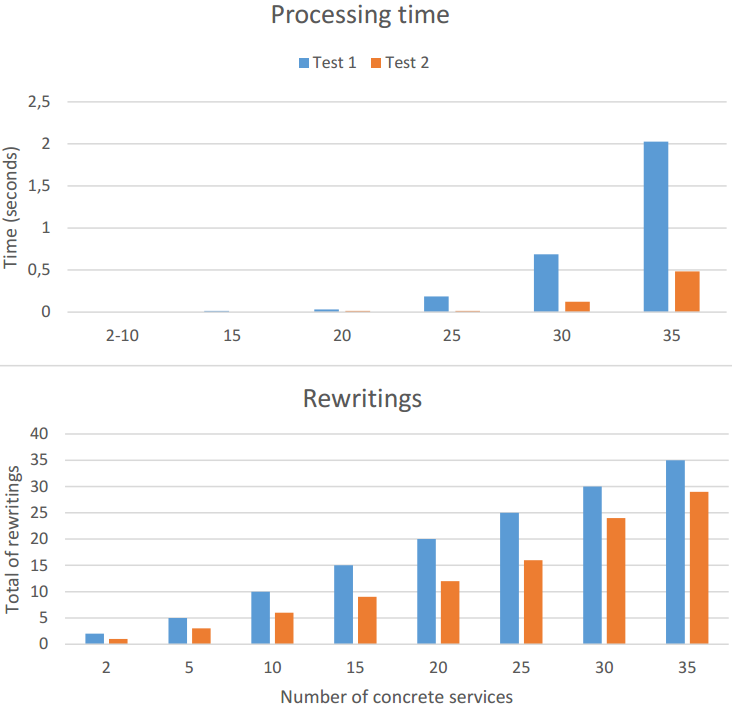
\includegraphics[scale=0.32]{analysis.png}
\label{fig:fig01}
\caption{Query rewriting evaluation.}
\end{figure} 
 
The analysis identified the algorithm shares the same problem as query rewriting approaches using views
(database domain) while it does not take into account quality measures (\textit{Test 1}): 
increasing the processing time when the query and the number of concrete services increase. 
However, while considering the quality measures (\textit{Test 2}), the results are promisingly.  
The \textit{Rhone} presents a better performance, decreasing the processing time and 
the total number of rewritings produced.  

%By now, the analysis identified that the factor that influenciates the Rhone
%performance is the number of CSDs versus the number of abstract services in the
%query since they increase the number of possible combinations of CSDs.  
%We proceeded two types of analysis for the query $Q$ (\textit{Test 1} and
%\textit{Test 2} - Figure 1). The first set of tests doesn't consider quality measures,
%while the second consider the measures in the rewriting process. The number of
%concrete services used in the analysis is from 2 until 35 services. Our
%preliminary results show that our algorithm, considering the quality measures,
%presents a better result for performance and the total number of rewritings.    

%To illustrate our approach in the next section, consider the \textit{concrete
% services} in table~\ref{table:concreteservices}.

% \begin{table}[h!]
% \center
% \begin{tabular}{p{7cm}}
% \hline
% \begin{small} $S1 (a?, b!) := DiseaseInfectedPatients(a?, b!)$ \end{small}\\ 
% \begin{small} $[availability > 99\%, \ price \ per \ call = 0.2\$]$ \end{small}\\ 
% \hline 
% \begin{small} $S2 (a?, b!) := DiseaseInfectedPatients(a?, b!)$ \end{small}\\
% \begin{small} $[availability > 99\%, \ price \ per \ call = 0.1\$]$ \end{small}\\ 
% \hline 
% \begin{small} $S3 (a?, b!, c!) := DiseaseInfectedPatients(a?, b!, c!)$ \end{small}\\
% \begin{small} $[availability > 98\%, \ price \ per \ call = 0.1\$]$ \end{small}\\ 
% \hline 
% \begin{small} $S4 (a?, b!) := PatientDNA(a?, b!)$ \end{small}\\
% \begin{small} $[availability > 99.5\%, \ price \ per \ call = 0.1\$]$ \end{small}\\ 
% \hline
% \begin{small} $S5 (a?, b!) := PatientDNA(a?, b!)$ \end{small}\\
% \begin{small} $[availability > 99.7\%, \ price \ per \ call = 0.1\$]$ \end{small}\\ 
% \hline
% \begin{small} $S6 (a?, b!) := PatientInformation(a?, b!)$ \end{small} \\
% \begin{small} $[availability > 99.7\%, \ price \ per \ call = 0.1\$]$ \end{small}\\ 
% \hline
% \begin{small} $S7 (a?, b!) := PatientDNA(a?, c!),PatientInformation(c?, b!)$ \end{small}\\
% \begin{small} $[availability > 99.7\%, \ price \ per \ call = 0.1\$]$ \end{small}\\ 
% \hline
% \end{tabular} \caption{Available \textit{concrete services}}
% \end{table}\label{table:concreteservices}

%\section{Implementation and Results}
The algorithm is implemented in Java. 
We are currently performing experiments in order to evaluate the performance of the Rhone. 
%To perform this, a set of testcases have been produced varying the number of concrete services, CSDs, abstract services and measures. 
The figure~\ref{figure:chart1} is an example of the charts we have created.
In this example all the queries have 6 \textit{abstract services} and 2 \textit{single measures}. The number of local variables (dependencies) and CSDs is being modified to see how the algorithm works under these conditions.
\begin{center}
\begin{figure}[h!]
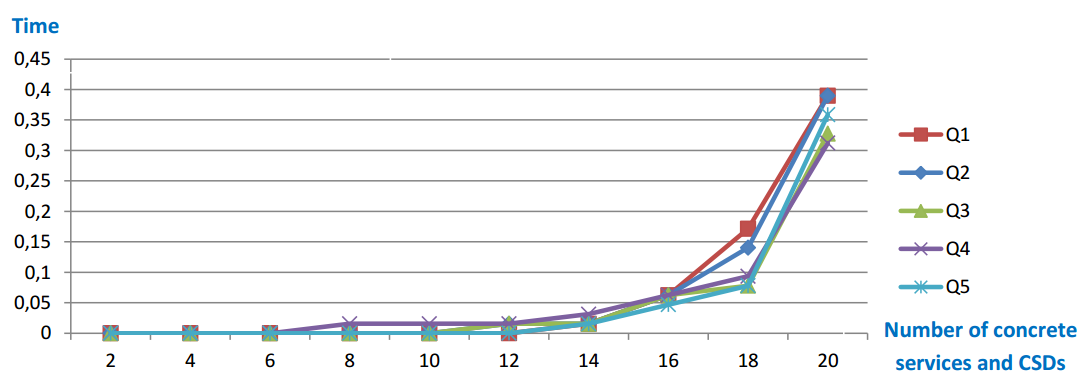
\includegraphics[scale=0.3]{chart1.PNG} 
\end{figure}\label{figure:chart1}
\end{center}

By now, the analysis identified that the factor that influenciates the Rhone performance is the number of CSDs vs. the number of abstract services in the query since they increase the number of possible combinations of CSDs.
 
\section{Conclusions}
\label{sec:conclusions}
%
%\begin{figure}[h!]
%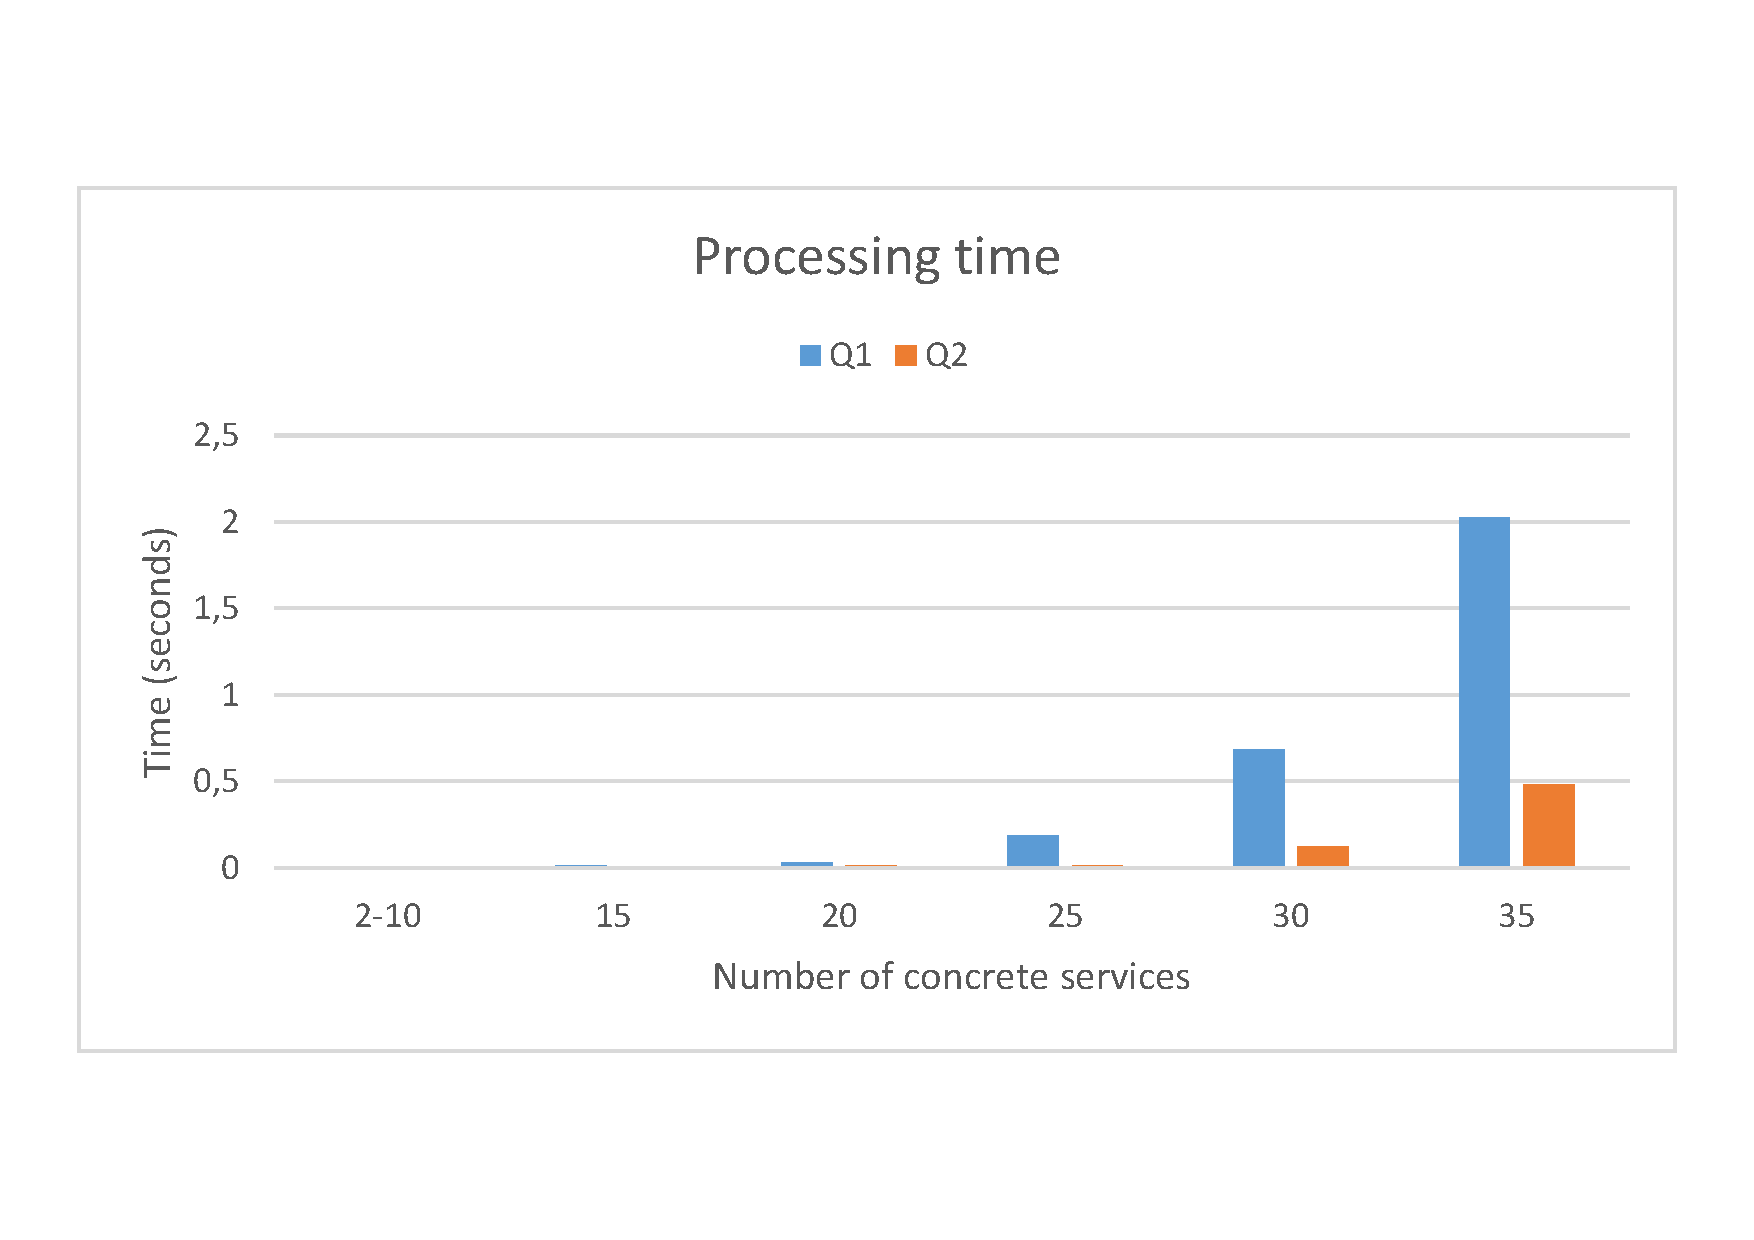
\includegraphics[scale=0.3]{fig2.pdf} 
%\end{figure}
%
%\begin{figure}[h!]
%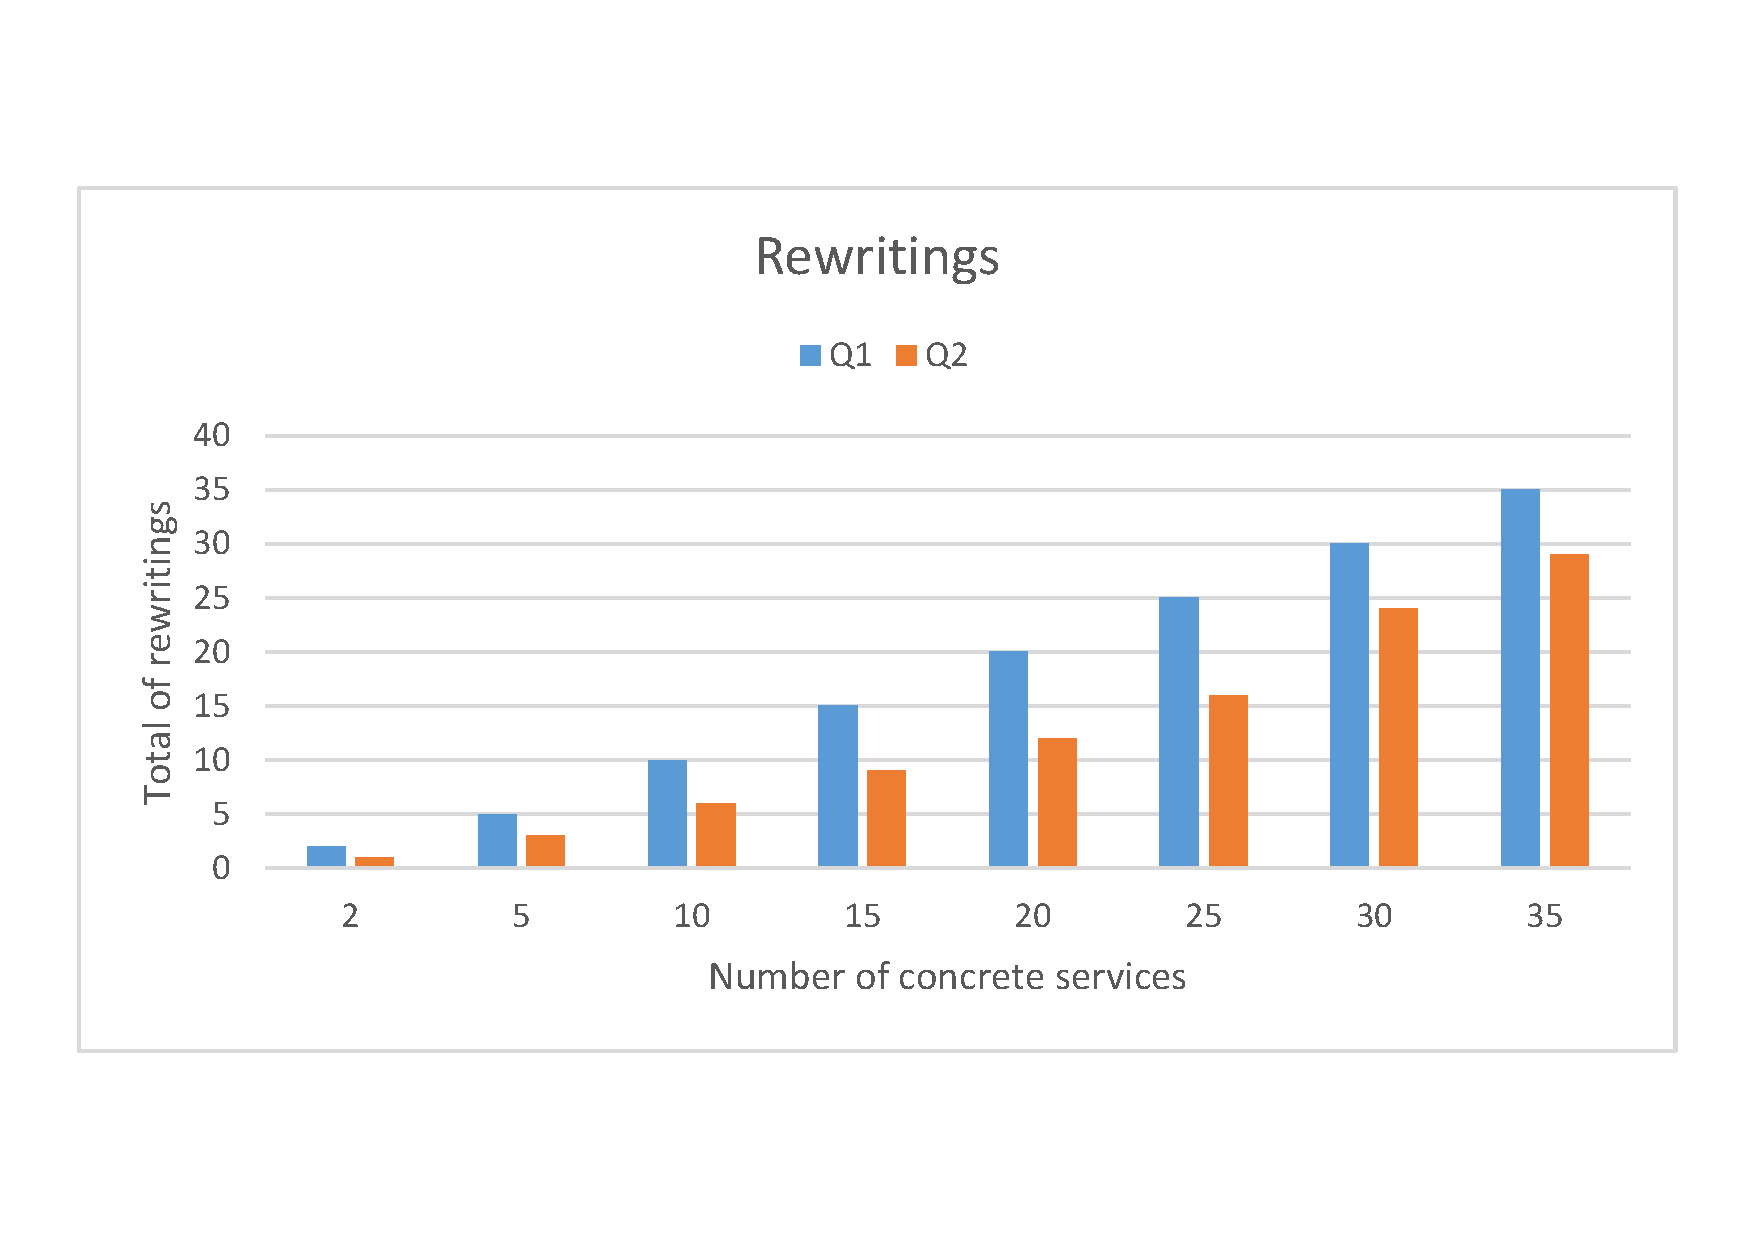
\includegraphics[scale=0.3]{fig1.pdf} 
%\end{figure}
 
This work proposes a query rewriting algorithm for data integration quality
named \textit{Rhone}. Given a query and a list of concrete services as input,
the algorithm looks for candidate concrete services. These candidate services can be used probably in the rewriting
process to match the query. We are currently performing experiments in order to
better evaluate the performance of the \textit{Rhone}.
%The algorithm is implemented in Java and w\ldots
% \ldots considering different sets of services in a multi-cloud environment.
%
%ACKNOWLEDGMENTS are optional
%\section{Acknowledgments}
%optional..
%
%
% The following two commands are all you need in the
% initial runs of your .tex file to
% produce the bibliography for the citations in your paper.
%{\tiny\bibliographystyle{abbrv}
\bibliographystyle{abbrv}
{\small
\bibliography{bibliography}}

\end{document}
